\documentclass[border=10pt]{standalone}
\usepackage{tikz}
\usetikzlibrary{arrows.meta,calc,positioning}

\begin{document}
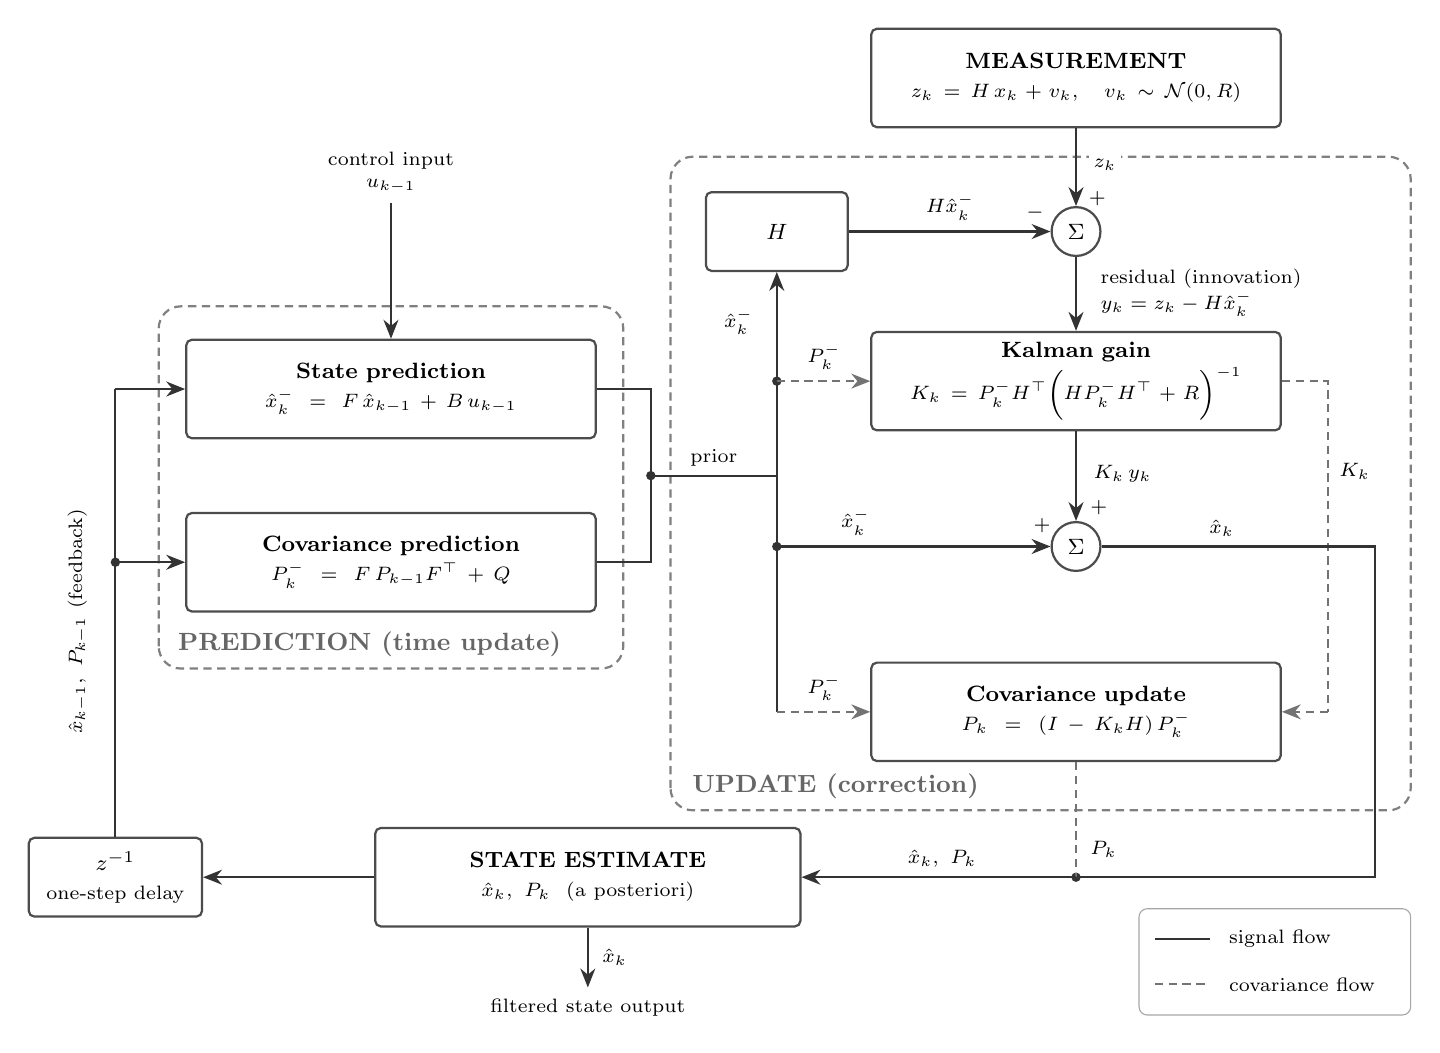
\begin{tikzpicture}[
  x=1cm, y=1cm,
  font=\footnotesize,
  block/.style={draw=black!70, thick, rounded corners=2pt, fill=white,
                minimum width=5.2cm, minimum height=1.25cm, text width=4.9cm,
                align=center, inner sep=3pt},
  gainblk/.style={draw=black!70, thick, rounded corners=2pt, fill=white,
                  minimum width=1.8cm, minimum height=1.0cm,
                  align=center, inner sep=2pt},
  sumnode/.style={draw=black!70, thick, circle, fill=white,
                  minimum size=0.62cm, inner sep=0pt},
  grp/.style={draw=black!50, thick, densely dashed, rounded corners=8pt},
  grplbl/.style={font=\small\bfseries, text=black!60, inner sep=2pt},
  sig/.style={draw=black!80, thick, -{Stealth[length=2.4mm,width=1.9mm]}},
  wire/.style={draw=black!80, thick},
  cov/.style={draw=black!55, thick, densely dashed,
              -{Stealth[length=2.4mm,width=1.9mm]}},
  covwire/.style={draw=black!55, thick, densely dashed},
  dot/.style={circle, fill=black!80, inner sep=0pt, minimum size=3.4pt},
  lbl/.style={font=\scriptsize, inner sep=1.6pt, fill=white, align=center},
  sgn/.style={font=\scriptsize, inner sep=1pt},
]

% ---------- group frames ----------
\draw[grp] (-2.95,-1.95) rectangle (2.95,2.65);
\node[grplbl, anchor=south west] at (-2.78,-1.88) {PREDICTION (time update)};

\draw[grp] (3.55,-3.75) rectangle (12.95,4.55);
\node[grplbl, anchor=south west] at (3.75,-3.68) {UPDATE (correction)};

% ---------- prediction blocks ----------
\node[block] (predA) at (0,1.6)
  {{\footnotesize\bfseries State prediction}\\[1pt]
   {\scriptsize $\hat{x}^{-}_{k} = F\,\hat{x}_{k-1} + B\,u_{k-1}$}};
\node[block] (predB) at (0,-0.6)
  {{\footnotesize\bfseries Covariance prediction}\\[1pt]
   {\scriptsize $P^{-}_{k} = F\,P_{k-1}F^{\top} + Q$}};

% ---------- measurement ----------
\node[block] (meas) at (8.7,5.55)
  {{\footnotesize\bfseries MEASUREMENT}\\[1pt]
   {\scriptsize $z_k = H\,x_k + v_k,\quad v_k \sim \mathcal{N}(0,R)$}};

% ---------- update blocks ----------
\node[gainblk] (hblk)  at (4.9,3.6) {$H$};
\node[sumnode] (sum1)  at (8.7,3.6) {$\Sigma$};
\node[block]   (kgain) at (8.7,1.7)
  {{\footnotesize\bfseries Kalman gain}\\[1pt]
   {\scriptsize $K_k = P^{-}_{k}H^{\top}\big(H P^{-}_{k}H^{\top} + R\big)^{-1}$}};
\node[sumnode] (sum2)  at (8.7,-0.4) {$\Sigma$};
\node[block]   (pupd)  at (8.7,-2.5)
  {{\footnotesize\bfseries Covariance update}\\[1pt]
   {\scriptsize $P_k = (I - K_k H)\,P^{-}_{k}$}};

% ---------- output / feedback ----------
\node[block, minimum width=5.4cm, text width=5.0cm] (est) at (2.5,-4.6)
  {{\footnotesize\bfseries STATE ESTIMATE}\\[1pt]
   {\scriptsize $\hat{x}_k,\ P_k$ \ (a posteriori)}};
\node[gainblk, minimum width=2.2cm] (delay) at (-3.5,-4.6)
  {$z^{-1}$\\[1pt]{\scriptsize one-step delay}};

% ---------- control input ----------
\node[font=\scriptsize, align=center] (uin) at (0,4.35)
  {control input\\ $u_{k-1}$};
\draw[sig] (uin.south) -- (predA.north);

% ---------- prior bus : prediction -> update ----------
\draw[wire] (predA.east) -- (3.3,1.6) -- (3.3,0.5);
\draw[wire] (predB.east) -- (3.3,-0.6) -- (3.3,0.5);
\node[dot] at (3.3,0.5) {};
\draw[wire] (3.3,0.5) -- (4.9,0.5);
\node[lbl, anchor=south] at (4.1,0.56) {prior};

\draw[wire] (4.9,-2.5) -- (4.9,0.5);
\draw[sig]  (4.9,0.5)  -- (hblk.south);
\node[lbl, anchor=east] at (4.66,2.45) {$\hat{x}^{-}_{k}$};

\node[dot] at (4.9,1.7) {};
\draw[cov] (4.9,1.7) -- (kgain.west);
\node[lbl, anchor=south] at (5.5,1.78) {$P^{-}_{k}$};

\node[dot] at (4.9,-0.4) {};
\draw[sig] (4.9,-0.4) -- (sum2.west);
\node[lbl, anchor=south] at (5.9,-0.32) {$\hat{x}^{-}_{k}$};

\draw[cov] (4.9,-2.5) -- (pupd.west);
\node[lbl, anchor=south] at (5.5,-2.42) {$P^{-}_{k}$};

% ---------- residual (innovation) ----------
\draw[sig] (hblk.east) -- (sum1.west);
\node[lbl, anchor=south] at (7.1,3.68) {$H\hat{x}^{-}_{k}$};
\node[sgn] at (8.18,3.84) {$-$};

\draw[sig] (meas.south) -- (sum1.north);
\node[lbl, anchor=west] at (8.86,4.45) {$z_k$};
\node[sgn] at (8.97,4.02) {$+$};

\draw[sig] (sum1.south) -- (kgain.north);
\node[lbl, anchor=west, align=left] at (8.95,2.82)
  {residual (innovation)\\ $y_k = z_k - H\hat{x}^{-}_{k}$};

% ---------- gain -> state correction ----------
\draw[sig] (kgain.south) -- (sum2.north);
\node[lbl, anchor=west] at (8.86,0.52) {$K_k\,y_k$};
\node[sgn] at (8.99,0.09) {$+$};
\node[sgn] at (8.27,-0.14) {$+$};

% ---------- gain -> covariance update ----------
\draw[covwire] (kgain.east) -- (11.9,1.7) -- (11.9,-2.5);
\draw[cov] (11.9,-2.5) -- (pupd.east);
\node[lbl, anchor=west] at (11.98,0.55) {$K_k$};

% ---------- posterior bus -> state estimate ----------
\draw[wire] (sum2.east) -- (12.5,-0.4) -- (12.5,-4.6) -- (8.7,-4.6);
\node[lbl, anchor=south] at (10.55,-0.34) {$\hat{x}_k$};
\node[dot] at (8.7,-4.6) {};
\draw[covwire] (pupd.south) -- (8.7,-4.6);
\node[lbl, anchor=west] at (8.82,-4.25) {$P_k$};
\draw[sig] (8.7,-4.6) -- (est.east);
\node[lbl, anchor=south] at (7.0,-4.54) {$\hat{x}_k,\ P_k$};

% ---------- filtered output ----------
\draw[sig] (est.south) -- (2.5,-6.0);
\node[lbl, anchor=west] at (2.62,-5.62) {$\hat{x}_k$};
\node[font=\scriptsize, anchor=north] at (2.5,-6.02) {filtered state output};

% ---------- feedback through unit delay ----------
\draw[sig] (est.west) -- (delay.east);
\draw[wire] (delay.north) -- (-3.5,1.6);
\node[dot] at (-3.5,-0.6) {};
\draw[sig] (-3.5,-0.6) -- (predB.west);
\draw[sig] (-3.5,1.6) -- (predA.west);
\node[lbl, rotate=90] at (-3.98,-1.35)
  {$\hat{x}_{k-1},\ P_{k-1}$ (feedback)};

% ---------- legend ----------
\draw[draw=black!35, rounded corners=3pt] (9.5,-6.35) rectangle (12.95,-5.0);
\draw[wire] (9.7,-5.38) -- (10.4,-5.38);
\node[font=\scriptsize, anchor=west] at (10.52,-5.38) {signal flow};
\draw[covwire] (9.7,-5.96) -- (10.4,-5.96);
\node[font=\scriptsize, anchor=west] at (10.52,-5.96) {covariance flow};

\end{tikzpicture}
\end{document}
